The goal was to maximize the twist rotation ($\phi$) in a backward somersault.
The model is composed of a 6-DoF root segment and two 1-DoF torque actuated arms.
The OCP was solved for two models.
First, rotations of the root segment were expressed as Euler angles.
They were expressed as a quaternion for the second model.
The objective functions were written as follow:

\begin{eqnarray}\label{eq:ocp_Trampo}
\mathcal{J} = -\underbrace{\int_0^T \dot{\phi}~dt}_{MINIMIZE\_TWIST}  +~\omega_1 \underbrace{\int_0^T \sum_{i=1}^{2}~\tau_{i}^2~dt}_{MINIMIZE\_ TORQUE},
\end{eqnarray}
with $\omega_1 = 1\times 10^{-6}$, T the duration of the movement and $\tau_{i}$ the torque control of the $i^{th}$ arm DoF.
The first term of the objective function (Eq.~\ref{eq:ocp_Trampo}) corresponds to maximizing the twist velocity and the second term is for control regularization.


The movement lasted for approximately 1 second and was discretized in 100 shooting nodes.
The solutions for both models were similar (Fig.~\ref{snapshots_quaternion_base_twisting_somersault}) highlighting the equivalence of the two rotation representations.
Euler angles have the advantage to be easily interpretable, but they suffer from the loss of a DoF at the gimbal lock.
The use of quaternion representation is advantageous for numerical stability when a joint is free to rotate on a wide three-dimensional range for motion.


\begin{figure*}[t!]
\centering
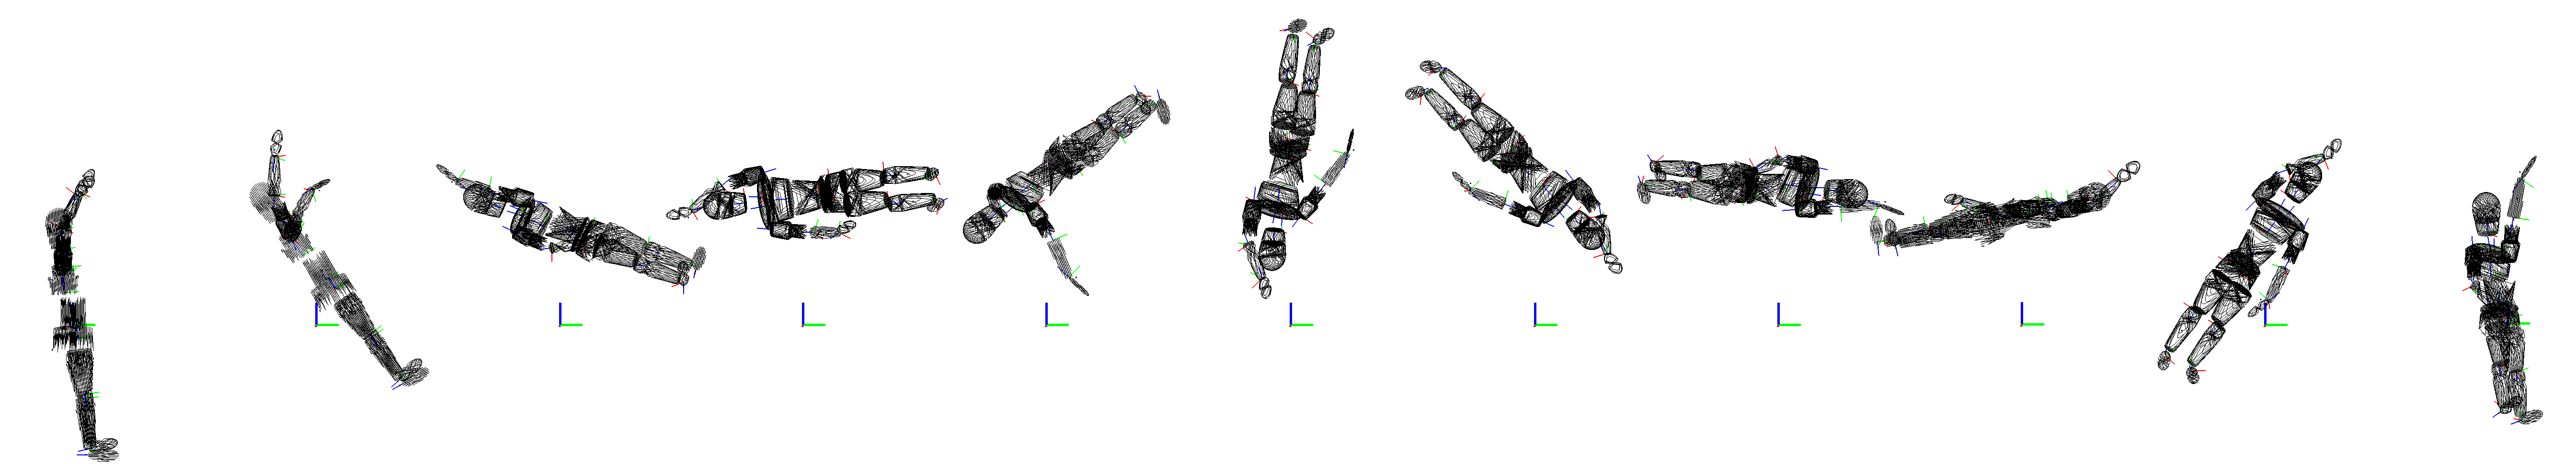
\includegraphics[width=\textwidth]{figures/Euler_Bioptim_MaxVrille_2.png}\\
\vspace*{0.5em}
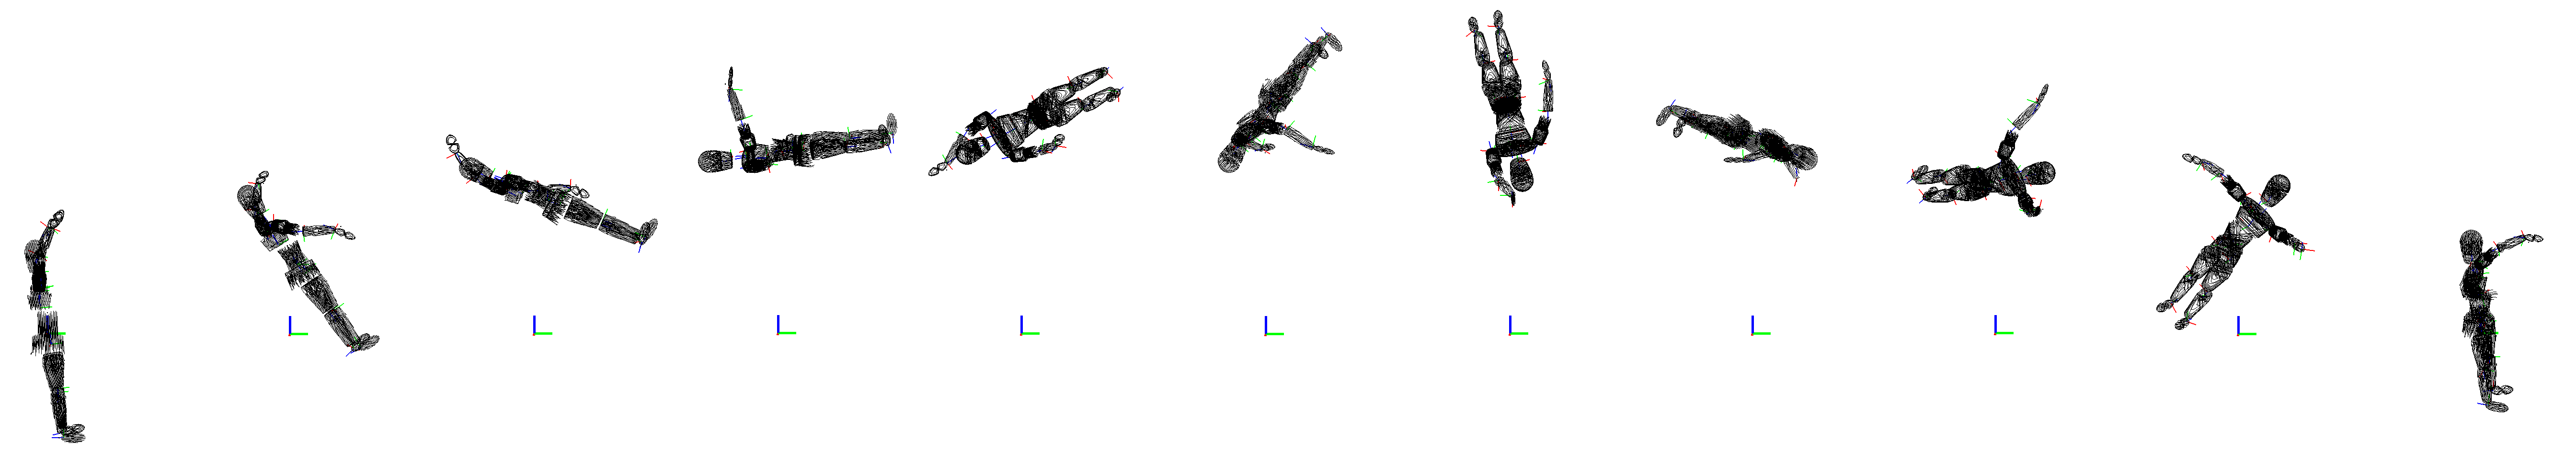
\includegraphics[width=\textwidth]{figures/Quat_Bioptim_MaxVrille_2.png}
\caption{Snapshots of a maximally twisting somersault driven by shoulder torque actuators and a free base expressed by Euler angles (top) or quaternions (bottom).}
\label{fig:snapshots_quaternion_base_twisting_somersault}
\end{figure*}


% \begin{table}[h!]
% \caption{\small Objective terms of quaternion base maximally twisting somersault}
% \label{tab:Quaternion_base_twisting_somersault}
% \centering
% \begin{tabular}{c c c c}
% \toprule 
% & Type & Function & Weight \\ 
% \midrule
% $\#1$ & Lagrange & MINIMIZE\_TWIST & $-1e1$ \\ 
% \midrule
% $\#2$ & Lagrange & MINIMIZE\_ TORQUE & $1e-6$ \\ 
% \bottomrule
% \end{tabular}
% \end{table}













